\documentclass[12pt]{article}
\usepackage{latexsym,amssymb,amsmath} 
\usepackage{cite}
\usepackage{path}
\usepackage{url}
\usepackage{verbatim}
\usepackage[pdftex]{graphicx}
\usepackage{fancyhdr}
\usepackage{hyperref}
\usepackage{booktabs}

\setlength{\oddsidemargin}{0.0in}
\setlength{\textwidth}{6.5in}
\setlength{\topmargin}{-1cm}
\setlength{\headheight}{12pt}
\setlength{\headsep}{25pt}
\setlength{\textheight}{625pt}
\setlength{\footskip}{24pt}

\renewcommand{\headrulewidth}{0pt}
\renewcommand{\textfraction}{0.10}
\renewcommand{\topfraction}{0.85}
\renewcommand{\bottomfraction}{0.85}
\renewcommand{\floatpagefraction}{0.90}

\numberwithin{equation}{section}
\numberwithin{table}{section}
\numberwithin{figure}{section}

\begin{document}
\DeclareGraphicsExtensions{.jpg}

%-------------------------Starts-------------------------------
\thispagestyle{fancy}
\rhead{$\mu$DBS Documentation}

\begin{center}
\textbf{\Large Process Fabrication for $\mu$DBS} \\[20pt]
  Daria Nesterovich\footnote{daria.nesterovich@utah.edu}\\[2pt] \emph{Salt Lake City, 84112, USA}  \\[6pt]
  (Dated: \today)
\end{center}

\vspace{6pt}


\begin{abstract}
The following content outlines the fabrication steps done in the Utah NanoFab Lab to build the $\mu$DBS. The purpose of this lab is to establish working recipes for the process and to keep track of past failures.
\end{abstract}

\section{Design Process Overview}

\subsection{Design Architecture}

The fabrication of the $\mu$DBS begins with design in Cadence through the X-FAB XC06 design package. The design is sent to X-FAB Foundry (Erfurt, GE) for fabrication. The chips that are returned must undergo metal plating for the contacts and the bond pads, a parylene coating, dicing, wire bonding, and assembly. The design architecture can be found in Figure~\ref{DesignArchitecture}

\section{General Instructions to Make a Mask}

\subsection{Lithography}
\begin{enumerate}
\item Use the \href{https://coral.nanofab.utah.edu/lab/equipment/show_eq/Heidelberg+MicroPG+101/}{Heidelberg MicroPG 101}
\item Click and follow instructions under the photolithography exposure wizard.
\item Record Size, Offset, Power (12 mW), Energy Mode (1/1). 
\item To make a positive mask, {\bf uncheck} inverted.
\end{enumerate}

\subsection{Exposure for mask}

\begin{enumerate}
\item AZ developer 1:1
\item Develop for 1 min, the run under rinse water
\item DI rinse - hit run
\item Dip for 3.5 min in Cr 14-S chromium etch
\item Rinse in DI for 2 min
\item Run in spin dryer (put in last spot)
\end{enumerate}
 
\section{General Instructions for Developing Photoresist}
 
\subsection{Applying Photoresist AZ 9260}
\begin{enumerate}
\item \href{https://coral.nanofab.utah.edu/lab/equipment/show_eq/CEE+100}{CEE 100 Spinner}
\item Spin at 2500 rpm, 60 Seconds
\item Bake at 110 C for 2+ Minutes
\end{enumerate}

\subsection{Exposing Photoresist AZ 9260}
\begin{enumerate}
\item Use the \href{https://coral.nanofab.utah.edu/lab/equipment/show_eq/EV+420}{EV 420 Aligner} 
\item 45 second exposure
\item 1:3.5 ratio of AZ 400K:DI water
\item 7 minute development
\item (FRESH BATCH EVERY TIME!!!!)
\end{enumerate}

\section{Creation of a Chip Tray} 

%% THICKNESS TABLE
\begin{table}[]
\centering
\caption{5" Wafer Thickness Measurements for Five Positions}\label{Thickness}
\begin{tabular}{@{}crrrrrr@{}}
\toprule
\multicolumn{7}{c}{\textbf{Wafer Thickness (mm)}}                                                                                                                                                                                                                           \\ \midrule
                    & \multicolumn{1}{c}{\textbf{Trial 1}} & \multicolumn{1}{c}{\textbf{Trial 2}} & \multicolumn{1}{c}{\textbf{Trial 3}} & \multicolumn{1}{c}{\textbf{Trial 4}} & \multicolumn{1}{c}{\textbf{Mean}} & \multicolumn{1}{c}{\textbf{SD}} \\
\textbf{Position 1} & 0.676 & 0.652 & 0.746 & 0.716 & 0.698 & 0.0417 \\
\textbf{Position 2} & 0.677 & 0.669 & 0.703 & 0.698 & 0.687 & 0.0163 \\
\textbf{Position 3} & 0.698 & 0.682 & 0.682 & 0.693 & 0.689 & 0.00806 \\
\textbf{Position 4} & 0.689 & 0.685 & 0.682 & 0.703 & 0.690 & 0.00929 \\
\textbf{Position 5} & 0.678 & 0.691 & 0.684 & 0.691 & 0.686 & 0.00627 \\ \bottomrule
\end{tabular}

\end{table}

%% LENGTH and WIDTH MEASUREMENT TABLE

\begin{table}[]
\centering
\caption{Proximal Length and Width Measurements }
\label{PLW}
\begin{tabular}{@{}crrrrrrrr@{}}
\toprule
\multicolumn{9}{c}{\textbf{Proximal Length and Width Measurements ($\mu$m)}}                                                                                                                                                                                                                                                                                   \\ \midrule
\multicolumn{1}{l}{} & \multicolumn{1}{c}{\textbf{Chip 1}} & \multicolumn{1}{c}{\textbf{Chip 2}} & \multicolumn{1}{c}{\textbf{Chip 3}} & \multicolumn{1}{c}{\textbf{Chip 4}} & \multicolumn{1}{c}{\textbf{Chip 5}} & \multicolumn{1}{c}{\textbf{Mean}} & \multicolumn{1}{c}{\textbf{SD}} & \multicolumn{1}{c}{\textbf{Mean + SD}} \\
\textbf{Position A}  & 1488  & 1490  & 1488  & 1490  & 1490 & 1489.2  & 1.10 & 1490.30 \\
\textbf{Position B}  & 1490  & 1492  & 1489  & 1488  & 1494 & 1490.6  & 2.41 & 1493.01 \\
\textbf{Position C}  & 1490  & 1489  & 1490  & 1488  & 1489 & 1489.2  & 0.84 & 1490.04 \\
\textbf{Position D}  & 10221 & 10224 & 10222 & 10218 & 10220 & 10221 & 2.24 & 10223.24 \\ \bottomrule
\end{tabular}
\end{table}

\begin{table}[]
\centering
\caption{Distal Length and Width Measurements }
\label{DLW}
\begin{tabular}{@{}crrrrrrrr@{}}
\toprule
\multicolumn{9}{c}{\textbf{Distal Length and Width Measurements ($\mu$m)}}                                                                                                                                                                                                                                                                                   \\ \midrule
\multicolumn{1}{l}{} & \multicolumn{1}{c}{\textbf{Chip 1}} & \multicolumn{1}{c}{\textbf{Chip 2}} & \multicolumn{1}{c}{\textbf{Chip 3}} & \multicolumn{1}{c}{\textbf{Chip 4}} & \multicolumn{1}{c}{\textbf{Chip 5}} & \multicolumn{1}{c}{\textbf{Mean}} & \multicolumn{1}{c}{\textbf{SD}} & \multicolumn{1}{c}{\textbf{Mean + SD}} \\
\textbf{Position A}  & 1493  & 1496  & 1495  & 1495  & 1494  & 1494.6  & 1.14 & 1495.74  \\
\textbf{Position B}  & 1494  & 1492  & 1494  & 1494  & 1492  & 1493.2  & 1.10 & 1494.30  \\
\textbf{Position C}  & 1495  & 1494  & 1492  & 1495  & 1495  & 1494.2  & 1.30 & 1495.50  \\ 
\textbf{Position D}  & 10220 & 10216 & 10217 & 10224 & 10221 & 10219.6 & 3.21 & 10222.81 \\ \bottomrule
\end{tabular}
\end{table}

%% OVERALL TABLES

\begin{table}[]
\centering
\caption{Length and Width Measurements for Proximal and Distal Chips}
\label{PDLW}
\begin{tabular}{@{}lrrrll|lrrr@{}}
\toprule
\multicolumn{4}{c}{\textbf{Proximal}} & \textbf{} & \textbf{} & \multicolumn{4}{c}{\textbf{Distal}} \\ \midrule
 & \multicolumn{1}{l}{\textbf{Mean}} & \multicolumn{1}{l}{\textbf{SD}} & \multicolumn{1}{l}{\textbf{Mean + SD}} & \textbf{} & \textbf{} &  & \multicolumn{1}{l}{\textbf{Mean}} & \multicolumn{1}{l}{\textbf{SD}} & \multicolumn{1}{l}{\textbf{Mean + SD}} \\
\textbf{Width} & 1489.67 & 1.63 & 1491.30 &  &  & \textbf{Width} & 1494 & 1.25 & 1495.25 \\
\textbf{Length} & 10221 & 2.24 & 10223.24 &  &  & \textbf{Length} & 10219.6 & 3.21 & 10222.81 \\ \bottomrule
\end{tabular}
\end{table}

\begin{table}[]
\centering
\caption{Overall Length and Width Measurements for Proximal and Distal Chips}
\label{OPDLW}
\begin{tabular}{@{}lrrr@{}}
\toprule
 & \multicolumn{1}{l}{\textbf{Overall Mean}} & \multicolumn{1}{l}{\textbf{Overall SD}} & \multicolumn{1}{l}{\textbf{Mean + SD}} \\ \midrule
\textbf{Width} & 1491.83 & 2.63 & 1494.46 \\
\textbf{Length} & 10220.3 & 2.71 & 10223.01 \\ \bottomrule
\end{tabular}
\end{table}

%% TEXT REGARDING MEASUREMENTS

\subsection{Measurements}
Thickness measurements were taken of a 5" wafer using the \href{https://coral.nanofab.utah.edu/lab/equipment/show_eq/Mitutoyo+Dial+Indicator+Probe}{Mitutoyo Dial Indicator Probe}. Results can be found in Table~\ref{Thickness}.
\\~\\
Measurements of 5 Proximal and 5 Distal chips were taken on the \href{https://coral.nanofab.utah.edu/lab/equipment/show_eq/Nikon+V12A}{Nikon V12A} microscope. Results can be found in Table~\ref{PLW} and Table~\ref{DLW}.
\\~\\
Length and width measurements can be found in Table~\ref{PDLW}.
\\~\\
Overall length and width measurements can be found in Table~\ref{OPDLW}.

\subsection{Mask Design}

%% TABLE FOR HEIDELBERG

\begin{table}[]
\centering
\caption{Run Parameters for Tray Mask}
\label{TM}
\begin{tabular}{@{}ll@{}}
\toprule
\multicolumn{2}{c}{\textbf{Heidelberg MicroPG 101 3 $\mu$m}} \\ \midrule
\multicolumn{2}{c}{\textbf{Run Parameters}} \\
\textbf{Design} & Tray\_Mask.gds \\
\textbf{Type / Scale} & gdsii / 1 \\
\textbf{Size X / Y ($\mu$m)} & 106667.9 / 106660.3 \\
\textbf{Offset X / Y ($\mu$m)} & 145 / 9.75 \\
\textbf{Power} & 12 mW \\
\textbf{Exposure Level} & 50\% \\
\textbf{Energy Mode} & 1x1 \\
\textbf{Inverted} & Uncheck \\
\textbf{Automatic Centering} & Check \\
\textbf{Auto Unload} & Check \\
\textbf{Stripes} & 13334 \\ \bottomrule
\end{tabular}
\end{table}

Run parameters for Tray Mask can be found in Table~\ref{TM}.

\begin{table}[]
\centering
\caption{My caption}
\label{my-label}
\begin{tabular}{@{}lr@{}}
\toprule
 & \multicolumn{1}{l}{\textbf{Measurement}} \\ \midrule
\textbf{A} & 1.464 \\
\textbf{B} & 1.469 \\
\textbf{C} & 1.467 \\
\textbf{D} & 10.193 \\ \bottomrule
\end{tabular}
\end{table}

 
\appendix

\section{Appendix 1} 
\label{appendix_1}

\begin{figure} \centering
  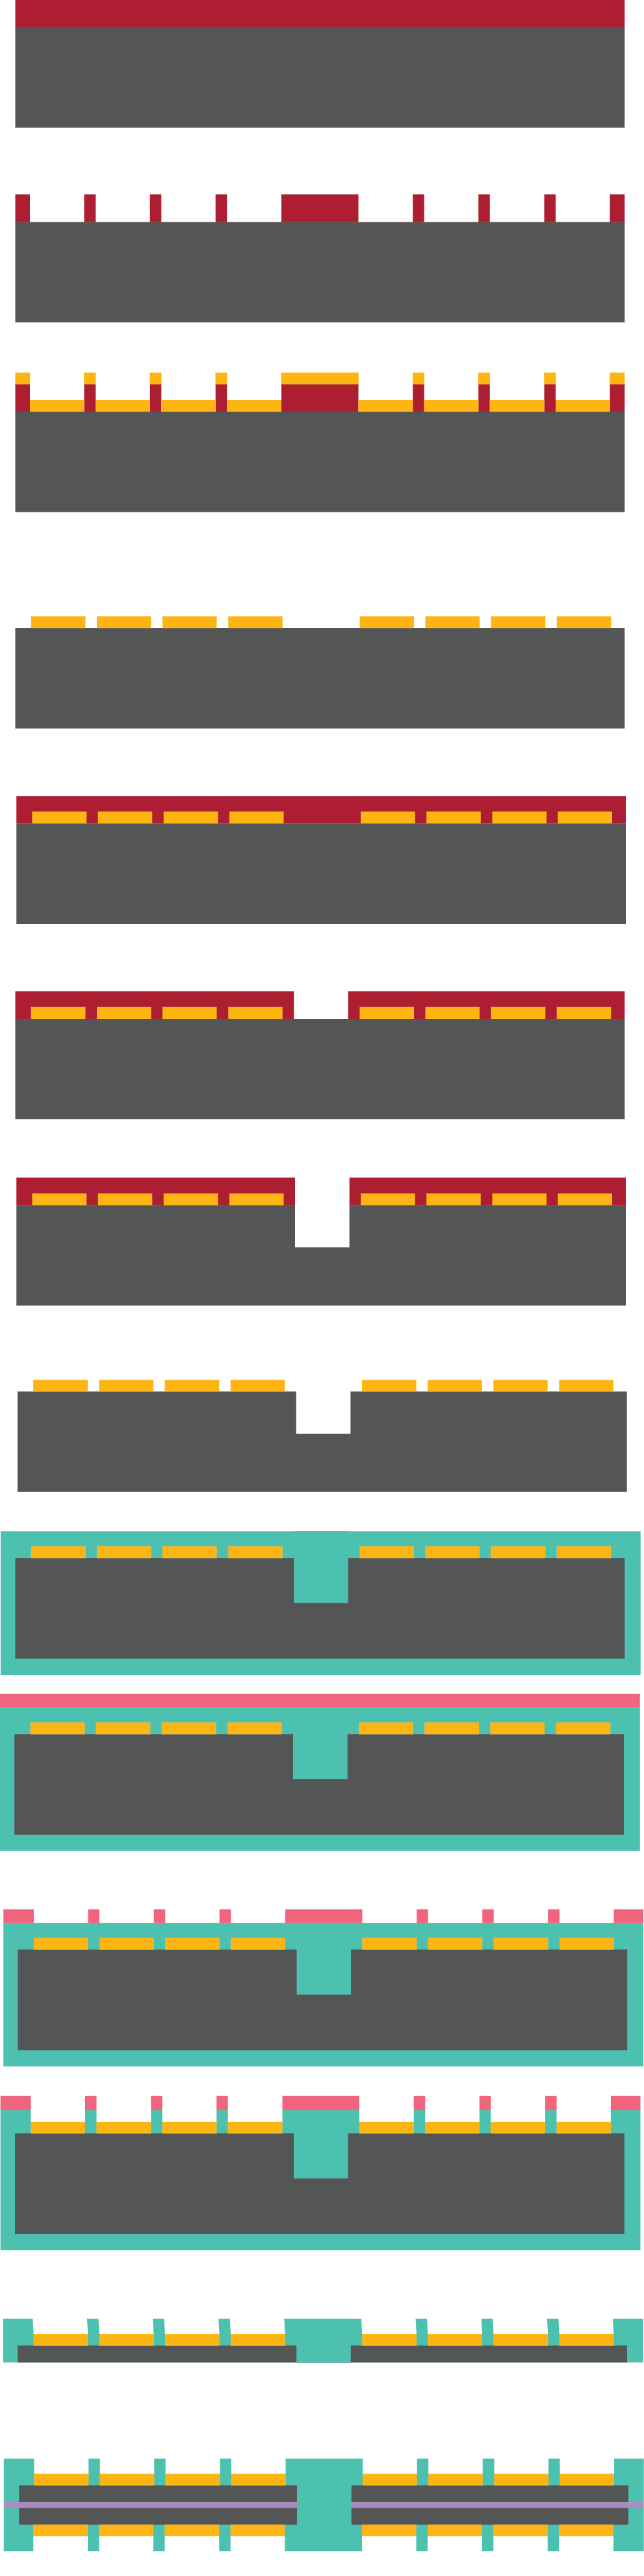
\includegraphics[width=0.25\textwidth]{DesignArchitecture.png}
  \caption{Design Architecture}
  \label{DesignArchitecture}
\end{figure}


%-------------------------Ends-------------------------------
\bibliographystyle{siam}
\bibliography{FermiTMtemp}

\end{document}

